% !TeX encoding = UTF-8
% !TeX spellcheck = en_US
% !TeX root = Presentation_AEDE8895_Spring2014.tex
% !TeX program = lualatex

\documentclass[svgnames]{beamer}

\usepackage{etex}


\usetheme{CambridgeUS}
\usecolortheme{dolphin}
%\useoutertheme{Randall}


%_________________________________________________________
%//////// FONTS //////////////////////////////////////////

%\usefonttheme{professionalfonts} % using non standard fonts for beamer
\usefonttheme{serif}
\usepackage{fontspec}
\setmainfont{Garamond} %{Goudy Old Style}
%\setmathfont{Neo Euler}

\usepackage{amsmath,amsfonts,mathtools,amssymb} % tools for typing mathematics
%\usepackage{unicode-math}
%\setmathfont[math-style=ISO]{Asana-Math}
\mathtoolsset{showonlyrefs}




\usepackage{graphicx}
\usepackage[update]{epstopdf}
\usepackage{framed}
\usepackage{xcolor}
%\usepackage[controls]{animate}
\usepackage{colortbl}
\usepackage{tabu}
\usepackage{wasysym}

\usepackage{verbatim}

\usepackage{hyperref}

\usepackage{tikz}
\usetikzlibrary{arrows,shapes}
%\usepackage[miktex]{gnuplottex}
%\usepackage{pgfplots}
\usepackage{fancybox}




\usepackage{rotating}
\def\Rot#1{\rlap{\rotatebox{90}{#1}~}}
\def\Rotate#1#2{\rlap{\rotatebox{#1}{#2}~}}



\DeclareMathOperator{\E}{\mathbb{E}}
\DeclareMathOperator{\R}{\mathbb{R}}
\DeclareMathOperator{\x}{\mathbf{x}}
\DeclareMathOperator{\h}{\mathbf{h}}
\DeclareMathOperator{\dd}{d\!}
\DeclareMathOperator{\Sy}{\mathbb{S}}
\usepackage{ctable}
%\newcolumntype{E}{>{$}l<{$}}

\graphicspath{{./Figures/}}


\input{/Users/Randall/LaTeX-Template/smart-column-blocks}
\input{/Users/Randall/LaTeX-Template/do-not-count-appendix-pages}


\AtBeginSection[]
{
  \begin{frame}<beamer>[plain,noframenumbering]{Outline}
    \tableofcontents[currentsection]
  \end{frame}
}
\setbeamertemplate{navigation symbols}{}


%/////////////////////  Bibliography ///////////////////////
\usepackage[%
bibstyle=authoryear,%
citestyle=authoryear,%
sorting=nyt,%
backend=biber,%
url=false,
doi=false,
]{biblatex} % to format the bibliography
\addbibresource{../oldBibtexDatabase.bib}






\setbeamercovered{%
still covered={\opaqueness<1->{5}},
again covered={\opaqueness<1->{40}}}






\begin{document}
\author[Romero-Aguilar]{Randall Romero-Aguilar}


\author[Romero-Aguilar, Miranda]{Randall Romero-Aguilar\hspace{3em} Mario J. Miranda\\ \vspace{1em}
	\includegraphics[scale=0.3]{OSU.png}}


\title[Food Security for Whom?]{Food Security for Whom?\\ \small{The Effectiveness of Food Reserves in Poor Developing Countries }}
\date[2014 AAEA Meeting]{2014 AAEA Annual Meeting\\Minneapolis, MN, July 27-29, 2014}




%\usebackgroundtemplate{%
%  \includegraphics[width=\paperwidth,height=\paperheight]{OSU-stadium.jpg}}

\begin{frame}[plain,noframenumbering] %titlepage
  \titlepage
\end{frame}




%===========================================================================


\section{Introduction}
\subsection{The problem}
%/////////////////////////////////////////////////////////////////////////
\begin{frame}
\frametitle{The Problem}
Despite rising production, food prices are higher and increasingly volatile\dots

\begin{figure}%\caption{FAO food price index}
\centering
\includegraphics[width=\linewidth]{FAO-cereals-price-BEAMER}    \\
\flushleft\tiny{Source: FAO's cereal price index}
\end{figure}
\end{frame}



%/////////////////////////////////////////////////////////////////////////
\begin{comment}
\begin{frame}[label=crisis-consequences]
\frametitle{\dots and its consequences}
\begin{columns}
\column{0.5\textwidth}
\begin{itemize}
\item<1> More price uncertainty $\Rightarrow$ increase in risk for farmers.
\item<2> Increase in hunger among poor net food buyers \dots
\begin{itemize}
\item<2> who account for 88\% of rural and 97\% of urban poor  households.
\end{itemize}
\item<3> More than 60 food riots in 30 different countries.

\end{itemize}
\column{0.5\textwidth}
\only<3>{
\includegraphics[width=\linewidth]{pic-food-riots}
}
\end{columns}
\end{frame}

\end{comment}





%/////////////////////////////////////////////////////////////////////////
\begin{frame}[label=hunger-estimates]
	\frametitle{Undernourished people in the world}
	\dots causing more (?) people to suffer hunger\dots
	\begin{figure}
		\centering
		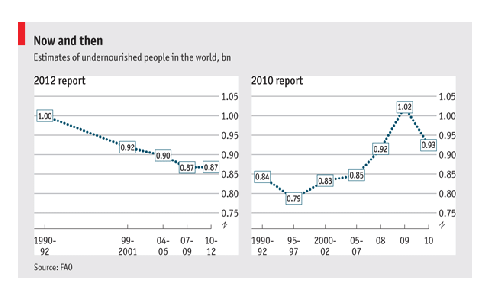
\includegraphics[width=0.95\textwidth]{fig-hunger-estimates.eps}
	\end{figure}
	\vspace{-1em}
	\tiny{Source: The Economist, Oct 10th 2012, based on FAO's SOFI reports.}
\end{frame}


%/////////////////////////////////////////////////////////////////////////
\begin{frame}[label=frame-riots]
\frametitle{Food riots}
\dots and in turn leading to increasing violence.
\vspace{-0.8em}
\begin{figure}
  \centering
  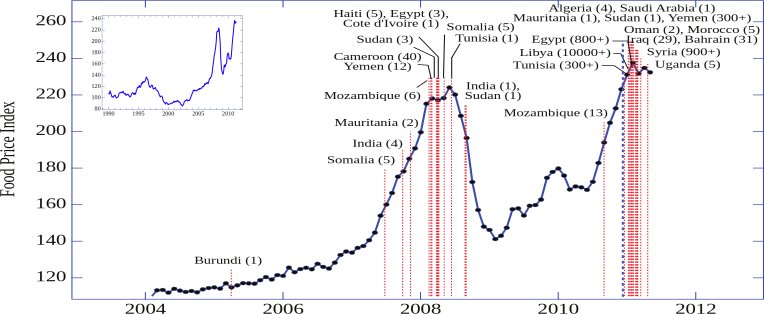
\includegraphics[width=0.9\textwidth]{fig-Lagi-et-al-food-riots.eps}
\end{figure}
\vspace{-1em}
 \tiny{Source: \cite{LagiBertrandBar-Yam:2011}} %\hyperlink{crisis-consequences}{\beamerreturnbutton}  \gotoLista
\end{frame}






\subsection{Food reserves}
%/////////////////////////////////////////////////////////////////////////
\begin{frame}
\frametitle{Food reserve as a solution?}
If a poor grain-importing country decides to operate a grain reserve to stabilize prices\dots
\begin{columns}
\column{0.65\textwidth}
\begin{itemize}[<+->]
\item what is the ultimate target: welfare vs.~hunger
\item what is the optimal size of the reserve?
\item is it better to use a financial asset?
\item \alert{how is the country's hunger rate affected by its operations?}
\end{itemize}
\column{0.35\textwidth}
\includegraphics[width=\linewidth]{pic-silos2}
\end{columns}
\end{frame}


%/////////////////////////////////////////////////////////////////////////
\begin{frame}
  \frametitle{Motivation: Is grain storage a good idea?}
  The logic behind grain storage is simple:
  \begin{itemize}
    \item<1-3> Seven years of abundance followed by seven years of famine\dots
    \item<2-3> What if country never has years of abundance?
    \item<3> Opportunity cost of storing grain is very high!
  \end{itemize}
  \vspace{2em}
  \only<4->{To answer this, a model should quantify }
  \begin{itemize}
    \item<5-> the increase on national hunger induced by an international crisis;
    \item<6-> to what extent a reserve alleviates this increase, and at \textcolor{red}{what cost}.
  \end{itemize}
\end{frame}



\section{The model}
\subsection{Main equations}
%/////////////////////////////////////////////////////////////////////////
\begin{frame}[label=essay1-key]
\frametitle{Key features of the model}
\begin{columns}
\column{0.6\textwidth}
\begin{itemize}
  \item<1> Nested utility: two goods, two food ingredients
  \item<2> Constant demand elasticities
  \item<3> Substitution between ingredients
  \item<4> Intertemporal, two grain prices
  \item<5> Heterogeneous households: log-logistic income distribution
  \item<6> Log-logistic food consumption  %\hyperlink{hunger-ECOWAS}{\beamergotobutton{data from ECOWAS}}
\end{itemize}

\column{0.4\textwidth}

\only<1>{
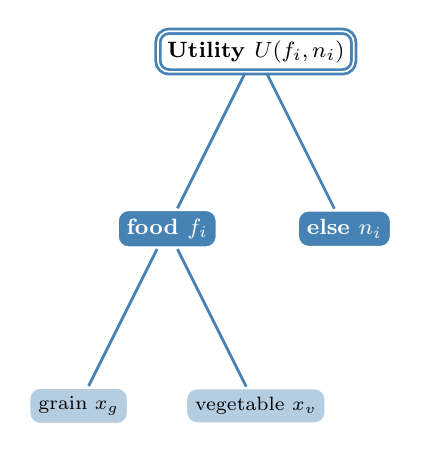
\begin{tikzpicture}  [scale = 1.5,line width = 1pt] % [level/.style={sibling distance=9cm}]
\node [color = SteelBlue,fill = white,text=black,double,draw,rounded corners] (a){\footnotesize \bf Utility $U(f_i,n_i)$} [grow = down]
[SteelBlue]
    child {node [color = white, fill = SteelBlue,text=white,draw,rounded corners] (b) {\footnotesize\bf food $f_i$} [grow = down]
       child{node [color = white, fill = SteelBlue!40!,text=black,draw,rounded corners] {\scriptsize grain $x_g$}}
       child [level distance = 15mm] {node [color = white, fill = SteelBlue!40!,text=black,draw,rounded corners] {\scriptsize vegetable $x_v$}}
    }
    child {node[color = white, fill = SteelBlue,text=white,draw,rounded corners] (c) {\footnotesize \bf else $n_i$}};
\end{tikzpicture}
}

\only<2>{
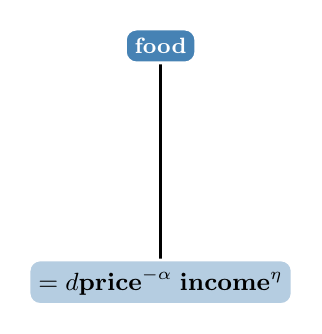
\begin{tikzpicture}  [scale = 2.0,line width = 1pt] % [level/.style={sibling distance=9cm}]
\node [color = white, fill = SteelBlue,text=white,draw,rounded corners] (b) {\footnotesize\bf food} [grow = down]
       child{node [color = white, fill = SteelBlue!40!,text=black,draw,rounded corners] {\small $=d\textbf{price}^{-\alpha}\;\textbf{income}^{\eta}$}};
\end{tikzpicture}
}

\only<3>{
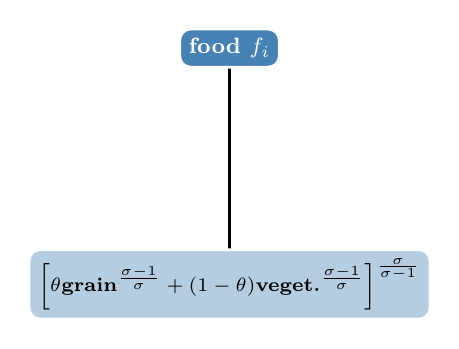
\begin{tikzpicture}  [scale = 2.0,line width = 1pt] % [level/.style={sibling distance=9cm}]
\node [color = white, fill = SteelBlue,text=white,draw,rounded corners] (b) {\footnotesize\bf food $f_i$} [grow = down]
       child{node [color = white, fill = SteelBlue!40!,text=black,draw,rounded corners] {\scriptsize $ \left[\theta \textbf{grain}^\frac{\sigma-1}{\sigma}+(1-\theta)\textbf{veget.}^\frac{\sigma-1}{\sigma}\right]^\frac{\sigma}{\sigma-1}$}};
\end{tikzpicture}
}
\end{columns}
\end{frame}


%/////////////////////////////////////////////////////////////////////////
\begin{frame}
\frametitle{Hunger changes in response to food prices}
\begin{equation}
  \Gamma(P) = \left[1+\left(\frac{cP^\alpha (G\pi)^\eta}{\zeta Y^\eta\sin^\eta(G\pi)}\right)^{1/{G\eta}}\right]^{-1}
\end{equation}


\begin{figure}
\centering
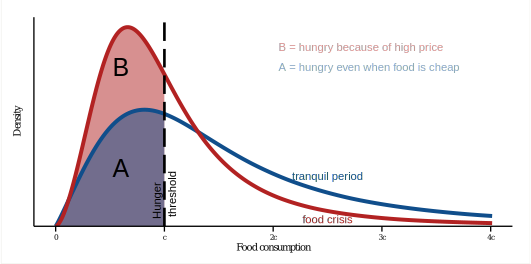
\includegraphics[width=\textwidth]{fig-Food-Distribution}
\end{figure}
\end{frame}




%/////////////////////////////////////////////////////////////////////////
\begin{frame}[label=essay1-gov]
\frametitle{Government problem: objectives and tools}
Government runs a grain stockpile to deal with price fluctuations.
\tikzstyle{every picture}+=[remember picture]

% By default all math in TikZ nodes are set in inline mode. Change this to
% displaystyle so that we don't get small fractions.
\everymath{\displaystyle}

\tikzstyle{na} = [baseline=-.5ex]

\begin{itemize}[<+-| alert@+>]
    \item Two alternative objectives:  \tikz[na] \node[coordinate] (n1) {}; welfare vs.\ hunger  %  \hyperlink{reward}{\beamergotobutton{details}}
    \item One policy tool:  \tikz[na]\node [coordinate] (n2) {}; tariff on grain imports
    \item Two state variables:  \tikz[na]\node [coordinate] (n3) {}; initial stock and grain price
\end{itemize}

% Below we mix an ordinary equation with TikZ nodes. Note that we have to
% adjust the baseline of the nodes to get proper alignment with the rest of
% the equation.
\begin{align*}
V\left(
        \tikz[baseline]{
            \node[fill=blue!20,anchor=base] (t1)
            {$ s,p_g^*$};
        }  \right) &=  \max_{
        \tikz[baseline]{
            \node[fill=red!20,anchor=base] (t2)
            {$\tau$};}
        } \left\{
        \tikz[baseline]{
            \node[fill=green!20,anchor=base] (t3)
            {$r(\tau,p_g^*)$};
        } + \delta \E V\left(s',{p_{g}^*}'\right)   \right\} \\ \\
       \uncover<3->{
       \text{subject to  } \quad
        \tikz[baseline]{
                   \node[fill=blue!20,anchor=base] (t5)
       {$s'$};
       }  & = (1-\phi)\left[s +\tfrac{1}{p_g^*} \Upsilon\left(
        \tikz[baseline]{
                   \node[fill=red!20,anchor=base] (t4){$\tau$};},
                   p_g^*\right) \right] \geq 0 \\ \\
        \pi_{ij} &= Pr\left({p_{g}^*}'= p_j\quad | \quad
                \tikz[baseline]{
                	\node[fill=blue!20,anchor=base] (t6)
                	{$p_{g}^*$};
                } = p_i\right)}
\end{align*}


% Now it's time to draw some edges between the global nodes. Note that we
% have to apply the 'overlay' style.
\begin{tikzpicture}[overlay]
        \path[->,dashed,green!90,very thick]<1> (n1) edge  [out=-90, in=90]  (t3);
        \path[->,dashed,red!60,very thick]<2> (n2) edge [out=-90, in=180] (t2);
        \path[->,dashed,red!60,very thick]<3> (t2) edge [out=-90, in=90] (t4);
        \path[->,dashed,blue!60,very thick]<3> (n3) edge [out=-90, in=90] (t1);
        \path[->,dashed,blue!60,very thick]<3> (t1) edge [out=-90, in=90] (t5);
        \path[->,dashed,blue!60,very thick]<3> (t5) edge [out=-90, in=90] (t6);
\end{tikzpicture}
%\only<3>{\hyperlink{solution}{\beamergotobutton{solution details}}}
\end{frame}


%/////////////////////////////////////////////////////////////////////////
\begin{frame}[label=reward]
	\frametitle{Reward function $r(\tau,P)$, by objective}
	\begin{table}
		\centering
		\begin{tabu} {X[-1c,m]X[2c,m]}
			\toprule
			Objective, $V$  &  Reward function, $r(\tau,\;p_g^*)$  \\  \midrule
			Hunger, $\Gamma$ & $
			\frac{1}{1-\rho}\left[1-\Gamma(\tau,p_g^*)\right]^{1-\rho} $  \\ \\
			Utility, $\Sy(v_i)$  &  \vspace{1em}$
			\frac{1}{1-\rho}\Sy\left[v(\tau,p_g^*)\right]^{1-\rho}  $ \\
			\bottomrule
		\end{tabu}
	\end{table}
\end{frame}

\subsection{Solution and parameterization}
%/////////////////////////////////////////////////////////////////////////
\begin{frame}
\frametitle{Solving the model: The food crisis in Haiti}
Calibration of parameters: Haiti
\begin{itemize}
  \item $\Gamma_{2011}=44.5\%$
  \item Imports $\approx 70\%$ of cereals consumed
  \item $p_g^*$ increased 85\% during crisis
\end{itemize}
\vspace{2em}
\uncover<2>{
\begin{columns}
\column{0.55\textwidth}
Food Crisis in Haiti:
\begin{itemize}
\item Dec2007-Mar2008: rice price doubles
\item Early April 2008: violent protests in Port-au-Prince
\item April 12: Prime Minister Jacques Adouard Alexis ousted
\end{itemize}
\column{0.45\textwidth}
\includegraphics<2>[width=\linewidth]{Figures/pic-haiti-riots}\\
\tiny{Residents protest on the streets in Port-au-Prince. Photograph: Eduardo Munoz/Reuters}
\end{columns}
}
\end{frame}


%/////////////////////////////////////////////////////////////////////////
\begin{frame}
\frametitle{Food reserve in Haiti}
\begin{itemize}
\item<1-> Jul2013: gov't begins construction of reserve, 35.000 tonnes
\vspace{1em}
\begin{figure}
\includegraphics[width=0.7\textwidth]{Haiti_building_reserve}
\end{figure}
\item<2> “The construction of this strategic reserve reflects the desire of my Government to promote national agricultural production, stabilize the market price of commodities and combat food insecurity. Indeed, the fight against hunger and extreme poverty constitutes the main pillars of government action.”
\end{itemize}\onslide<2>{\flushright\tiny{Prime Minister, Laurent Lamothe}}
\end{frame}



%/////////////////////////////////////////////////////////////////////////
\begin{frame}
\frametitle{Solving the model: Numerical methods}
\begin{itemize}
\item<1> Numerical solution:
\begin{itemize}
\item Collocation method  (\emph{dpsolve} solver in \emph{CompEcon})
\item Chebyshev polynomials with 12 nodes for continuous state $s_t$
\item One discrete variable, price, with values 1.0 and 1.85
\end{itemize}
\vspace{1.5em}
\item<2> Once solved, run Monte Carlo simulations to assess performance of the policy
\end{itemize}
\end{frame}

\begin{frame}
\frametitle{Baseline parameters}
\begin{footnotesize}
\begin{tabu} to \textwidth {X[c$ $]X[c]X[3.0l]}
    \tabucline[1.5pt]{-}
    \text{Parameter} & \multicolumn{1}{c}{Value} & Description  \\ \tabucline[0.75pt]{-}
    \input{Tables/table-parameters.tex} \\
 \tabucline[1.5pt]{-}
  \end{tabu}
\end{footnotesize}
\end{frame}


\section{Results}
\subsection{Without policy}
%/////////////////////////////////////////////////////////////////////////
\begin{frame}
\frametitle{The effects of crisis, without policy}
\centering

\begin{tabu} to 0.75\textwidth {X[4l]*2{X[1c]}*1{>{\columncolor{Black!10}}X[1c]}}
  Variable           & $p_L$ & $p_H$ & $\Delta\%$ \\ \midrule
  Price of grain     & 1.0   & 1.85 &  85.0 \\
  Price of food      & 1.0   & 1.25 &  25.5 \\
  Food consumption   & 50.8  & 42.5 & -16.4 \\
  Grain consumption  & 16.9  & 11.7 & -31.1 \\
  Vegetable consumption & 33.9  & 31.8 & - 6.3 \\
  \rowcolor{Blue!15}
  Hunger rate (\%)   & 44.5  & 53.8 &  20.8 \\
  \bottomrule
\end{tabu}
\end{frame}

\subsection{Optimal policy}
%/////////////////////////////////////////////////////////////////////////
\begin{frame}
\frametitle{Storage policy}
\centering
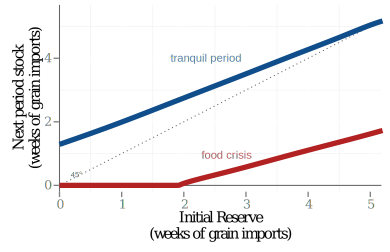
\includegraphics[width=\textwidth]{Storage-policy}
\end{frame}


%/////////////////////////////////////////////////////////////////////////
\begin{frame}[label=hunger-policy]
\frametitle{Effects of storage policy on hunger}
\centering
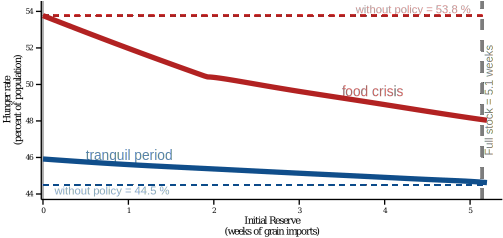
\includegraphics[width=\textwidth]{Hunger-policy}
\end{frame}


\subsection{Long-term simulations}
%/////////////////////////////////////////////////////////////////////////
\begin{frame}
\frametitle{Long-term distribution of grain reserve}
In half of the crisis, the reserve would be empty! \\
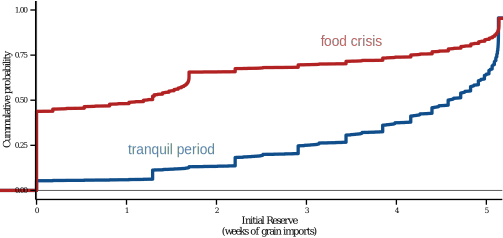
\includegraphics[width=\textwidth]{Storage-cdf}
\end{frame}


%/////////////////////////////////////////////////////////////////////////
\begin{frame}
\frametitle{Long-term distribution of hunger}
\small{The reserve would fail at preventing extreme hunger.}
\centering
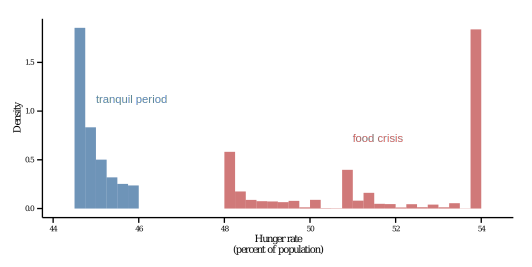
\includegraphics[width=\textwidth]{Hunger-histogram}
\end{frame}


\subsection{Alternatives to a food reserve}
%/////////////////////////////////////////////////////////////////////////
\begin{frame}
\frametitle{Cash vs. grain reserve?}
\begin{itemize}
\item \small{In this scenario, a grain reserve outperforms a cash reserve, but difference is small.}
\end{itemize}
\vspace{1em}
\centering
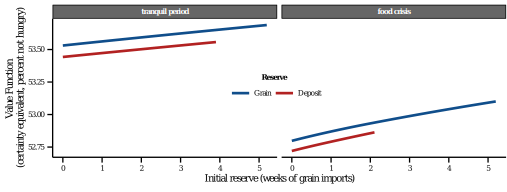
\includegraphics[width=\textwidth]{Value-function-facet-baseline}
\end{frame}


%/////////////////////////////////////////////////////////////////////////
\begin{frame}
\frametitle{Food storage vs. fighting poverty}
\begin{itemize}
\item \small{Resources used for grain reserve might be better spent at promoting growth.}
\end{itemize}
\vspace{1em}
\centering
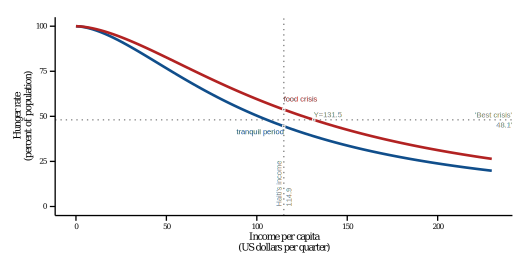
\includegraphics[width=\textwidth]{fig-Effect-Income}
\end{frame}


%/////////////////////////////////////////////////////////////////////////
\begin{frame}
\frametitle{Price stabilization vs. safety net?}
\begin{itemize}
\item  \small{Income redistribution, targeting the poor, may have a better outcome.}
\end{itemize}
\vspace{1em}
\centering
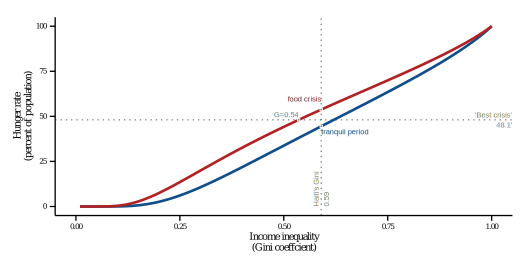
\includegraphics[width=\textwidth]{fig-Effect-Inequality}
\end{frame}







\section{Conclusions}
%/////////////////////////////////////////////////////////////////////////
\begin{frame}
\frametitle{Conclusions}
\setbeamercovered{%
still covered={\opaqueness<1->{5}},
again covered={\opaqueness<1->{40}}}
The optimal grain storage policy\dots
  \begin{itemize}
    \item<1> would not fully stabilize food prices.
    \item<2> would not prevent extreme hunger, yet it would reduce its frequency.
    \item<3> is very sensitive to key parameters (price process, storage costs)
    \item<4> might be outperformed by policies that attack poverty directly.
    \item<5> in many cases, no better than accumulating financial assets.
    \item<6> is more “active” when objective is avoiding extreme hunger.
  \end{itemize}
\end{frame}


\beginbackup
\section*{Appendix}

\begin{frame}[fragile]
\frametitle{References}
\printbibliography
\end{frame}


%/////////////////////////////////////////////////////////////////////////
\begin{frame}[label=frame-causes-crisis]
\frametitle{Possible causes of high food prices}
\begin{columns}
\column{0.5\textwidth}
Affecting supply:
\begin{enumerate}
  \item rising oil prices;
  \item declining stocks and reserves;
  \item regional catastrophic weather;
  \item export restrictions;
  \item decline in productivity and R\&D in agriculture.
\end{enumerate}


\column{0.5\textwidth}
Affecting demand:
\begin{enumerate}
  \item strong income growth in China and India;
  \item biofuel production in the USA and Europe;
  \item preventive imports surges;
  \item speculation in financial markets.
\end{enumerate}
\end{columns}
\end{frame}



%/////////////////////////////////////////////////////////////////////////
\begin{frame}[label=hunger-ECOWAS]
\frametitle{Empirical relevance of the model}
\framesubtitle{Food adequacy $x_{it}$ and undernourishment $\Gamma_{it}$ in ECOWAS and ASEAN}
\begin{equation}
   \log\left(\tfrac{\Gamma_{it}}{1-\Gamma_{it}}\right) = d_i^* - b_f\log x_{it} +  \epsilon_{it}
\end{equation}
\begin{columns}
  \column{0.25\textwidth}
  \small{Model approximates FAO's hunger estimates reasonably well.}
  \scriptsize{
  \begin{itemize}
    \item FAO data
    \item Fixed-effects
    \item 1991-2011
  \end{itemize}
  }

  \column{0.75\textwidth}
  \only<1>{\centering ECOWAS countries\\
  \includegraphics[width=0.95\textwidth]{fig-Regression-adjusted-ECOWAS12.eps}\\ %\hyperlink{essay1-key<6>}{\beamerreturnbutton}  \gotoLista
  }
  \only<2>{\centering ASEAN countries\\
  \includegraphics[width=0.95\textwidth]{fig-Regression-adjusted-ASEAN.eps} %\hyperlink{essay1-key<6>}{\beamerreturnbutton}  \gotoLista
  }
\end{columns}
\end{frame}


\begin{frame}
\frametitle{Alternative scenarios}
\begin{description}
\item[1] Baseline
\item[2] Increased risk aversion, from $\rho=2.5$ to $\rho=3.0$
\item[3] Crisis expected to last $\psi=4$ quarters,  instead of $\psi=3$
\item[4] Double the cost of storage, $\phi=0.05$
\item[5] Less severe crisis: $p^*_g=1.6$ instead of 1.85
\end{description}
\end{frame}


%/////////////////////////////////////////////////////////////////////////
\begin{frame}
\frametitle{Summary statistics for other scenarios}
\begin{tiny}
\begin{tabu} {*1{X[1c]}*1{>{\columncolor{SteelBlue!40}}X[1c]}*1{X[1c]}*1{>{\columncolor{SteelBlue!40}}X[1c]}*1{X[1c]}} \savetabu{fiveDoubleColumns} \end{tabu}
\begin{tabu} {*2{X[1c]}*2{>{\columncolor{SteelBlue!20}}X[1c]}*2{X[1c]}*2{>{\columncolor{SteelBlue!20}}X[1c]}*2{X[1c]}} \savetabu{tenColumns} \end{tabu}

  \begin{tabu} to 1.05\textwidth {>{\color{white}\columncolor{SteelBlue}}X[1,c,m]>{\columncolor{SteelBlue!40}}X[0.5,c,m] X[12,c,m]}
   \cellcolor{white}& \cellcolor{white}  &
    \begin{tabu} {\preamble{fiveDoubleColumns}}
    Scenario 1:  & Scenario 2: & Scenario 3: & Scenario 4: & Scenario 5:  \\
  	  (baseline) & $\rho=3.0$  & $\psi=4$    & $\phi=0.05$ & $P_H= 1.60$   \\
  \end{tabu} \\ \midrule [0.4pt]
% HEADINGS*************************************************************
  {Variable}  & {Stat.}  &
   \begin{tabu} {\preamble{tenColumns}}
   $p_L$ & $p_H$ & $p_L$ & $p_H$ & $p_L$ & $p_H$ & $p_L$ & $p_H$ & $p_L$ & $p_H$
   \end{tabu} \\  \midrule [1pt]
% STATISTICS BLOCK****************************************************************
Tax rate, \%    & \input{Tables/taInd.tex} & \input{Tables/table-Tax.tex}           \\ \midrule
Initial stock   & \input{Tables/taInd.tex} & \input{Tables/table-InitialStockN.tex} \\ \midrule
End stock       & \input{Tables/taInd.tex} & \input{Tables/table-StockN.tex}        \\ \midrule
Food price      & \input{Tables/taInd.tex} & \input{Tables/table-FoodPrice.tex}     \\ \midrule
Hunger rate, \% & \input{Tables/taInd.tex} & \input{Tables/table-Hunger.tex}        \\ \bottomrule
  \end{tabu}
  \end{tiny}
\end{frame}



%/////////////////////////////////////////////////////////////////////////
%\begin{frame}[plain]
%\centering
%\includegraphics[width=0.9\linewidth]{Hunger-histogram-facet}
%\end{frame}


%/////////////////////////////////////////////////////////////////////////
\begin{frame}[label=frame-export-restrictions]
	\frametitle{The effects of export restrictions on rice prices}
	\begin{figure}
		\centering
		\includegraphics[width=0.9\textwidth]{fig_rice-price-and-restrictions.eps}
	\end{figure}
	\vspace{-2em}
	\tiny{Source: \textcite{Headey:2011a}}
\end{frame}




\backupend
\end{document} 